Given a generative model over $x$ and $y$ paramitised with $\theta$, we are dealing with the joint distribution
$$p(x,y|\theta)$$
and we are interested in the condtional distribution of y given x, 
$$p(y|x, \theta_{y|x})$$
where we have put subscript on $\theta$ in order to jump up a level of abstraction since, 
in fact there is just a mapping between them $\theta_{y|x} := g(\theta, y, x)$ 

% $$\alpha p(y|x) + (1-\alpha) \mathcal{N}(0,1)$$

% so what should $\alpha$ be? Here we can find inspiration from a Poission point process. 


\begin{align*}
    p(y|x, \mathcal{D}) &= \int p(y|x,\theta_{y|x})p(\theta_{y|x}|\mathcal{D}) d\theta_{y|x}  \\
    &=  p(y|x,\hat \theta_{y|x})
\end{align*}
Where the last equation holds as we assume that $p(\theta_{y|x}|\mathcal{D})$ is a delta function
i.e. a point estimate with value $\hat \theta_{y|x}$. In the case of our Gaussian mixture model, 
we obtain a point estiamte from the EM algorithm for the variance $\Sigma_{y|k}$, mean value $\mu_{y|k}$ and proportion $\pi_{y|k}$
for each component $k = 1,2, \dots, K$
$$\hat \theta_{y|x} = (\hat\Sigma_{y|k}, \hat\mu_{y|k}, \hat\pi_{y|k})_{k=1}^K$$

However, we are not satisfied with the variance estimate for the regression, as it is way too small for areas with
no observed data. It is therefore necessary to manipulate the variance estimate accoring to that observation. 
We multiply the variance obtained using expectation-maximization on the joint distribution with the 
inverse of the probability of the data $x$, and control that the scaling factor is not going wild!

$$\hat\Sigma_{y|k} =\Sigma_{y|k}^{GMM} \frac{1}{\max(p(x), 0.01)}$$

In a way, this is manipulation in a Bayesian spirit, as we let prior and subjective knowledge influence the
variance prediction. 
\subsection{Inclusion of prior distribution}
The new conditional distribution is essentially a mixture between the old conditional and the prior distribution, 
$$\hat p(y|x) = \alpha_x p(y|x) + (1-\alpha_x)p_{prior}(y)$$
where we choose $\alpha_x := \frac{S(x)}{S(x)+1}$. A convex combination of distributions is a distribution, 
since 
\begin{align*}
    \int_y \hat p(y|x) dy &= \int_y \left[ \alpha_x p(y|x) + (1-\alpha_x)p_{prior}(y) \right] dy\\
     &= \alpha_x \int_y p(y|x)dy +(1-\alpha_x) \int_y p_{prior}(y)dy \\
     &= \alpha_x + (1-\alpha_x) = 1
\end{align*}
    
\subsection{Inclusion of prior distribution}
Since the prior predictive distribution and the predictive distribution both are assumed to be normal distributions, 
it is possible to simply let the parameters of the manipulated predictive distributions be a convex combination of the 
parameters. This will make the manipulation be more natural, and hopefully less coruptive. 
\begin{align*}
    \hat p (y|x) &=\mathcal{N}(y| \hat \mu, \hat\sigma^2)\\
    \hat \mu &= \alpha \cdot \mu_{y|x} + (1-\alpha) \cdot \mu_{prior}\\
    \hat \sigma^2 &= \alpha \cdot \sigma_{y|x}^2 + (1-\alpha) \cdot\sigma_{prior}^2
\end{align*}


\subsection{Inclusion of prior distribution}
The conditional distribution $p(y|x)$ obtained from using a Gaussian mixture model is without a prior, and
the predictive distribution yields a way too small uncertainty estimate in regions where there are no observations.
This is because the range of the Gaussian distribution continues throughout the entire space and even though the
joint distribution is very small in the region, the conditional distribution is normalized using the (very small) $p(x)$.
We, therefore, want to introduce a prior, which can rule over the conditional in regions where the probability is too
small. The first approach is simply to define a new conditional distribution, 
\begin{align}\label{manipulated_pred_dist}
    \hat p(y|x) &\propto S(x) \cdot p(y|x) + p_{prior}(y)
\end{align}
where the scaling function can be interpreted as the probability of the input $x$ is in the region
ball $x \in B_{\frac{1}{2}\Delta}(x)$, and the probability density is not just $p(x)$ but the
probability of the average mixture component, which is $K\cdot p(x)$, assuming the mixture is
dominated be a single component at the position $x$. We define the scaling as 
$$S(x):= K\cdot p(x)\cdot \Delta$$
% $p_K(x)$ is the marginal density of an average mixture component, i.e. 
% $$p(x) = \sum_{k=1}^K \gamma_k p_k(x) \implies p_K(x) = K \cdot p(x)$$
Next we need to normalize the manipulated predictive distribution in order to
make it a proper probability density, i.e., making sure it integrates to 1, 
$$\int S(x) \cdot p(y|x) + p_{prior}(y) dy =S(x)+1$$
so the we can easily update \eqref{manipulated_pred_dist} with an equality
sign by defining the manipulated predive distribution as, 
$$\hat p(y|x) = \frac{S(x) \cdot p(y|x) + p_{prior}(y)}{S(x)+1}.$$

In figure \ref{pred_dist_manipulation} the manipulated predictive 
distribution is illustrated under the influenced of different scalings. 
Note that if $S(x) = 0$ the manipulated distribution becomes the prior,
while in the limit $S(x) \rightarrow \infty$ the manipulated distribution
become the original predictive distribtuion, $\hat p(y|x) = p(y|x)$. 

\begin{figure}[H]
    \centering
    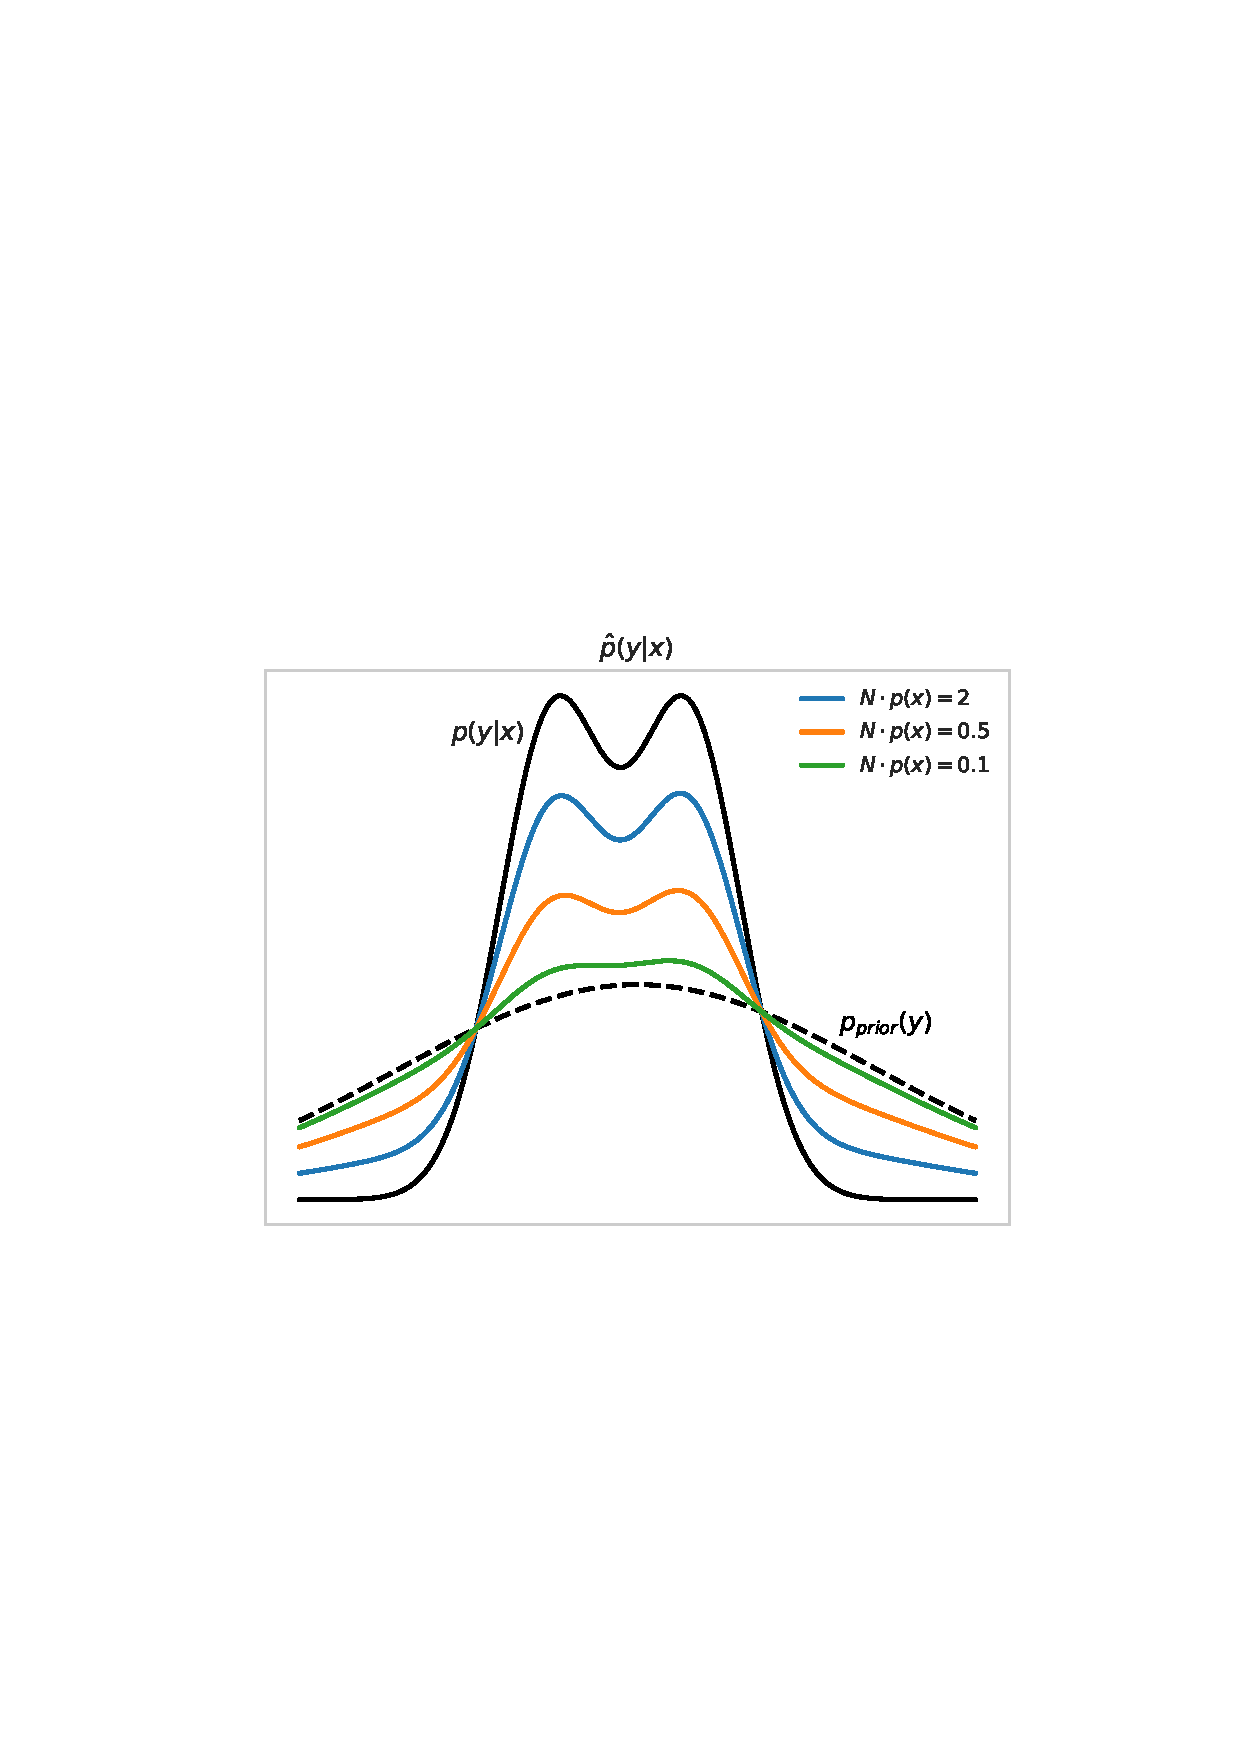
\includegraphics[width=0.45\textwidth]{Pictures/mixture_predictive_bayesian.pdf}
    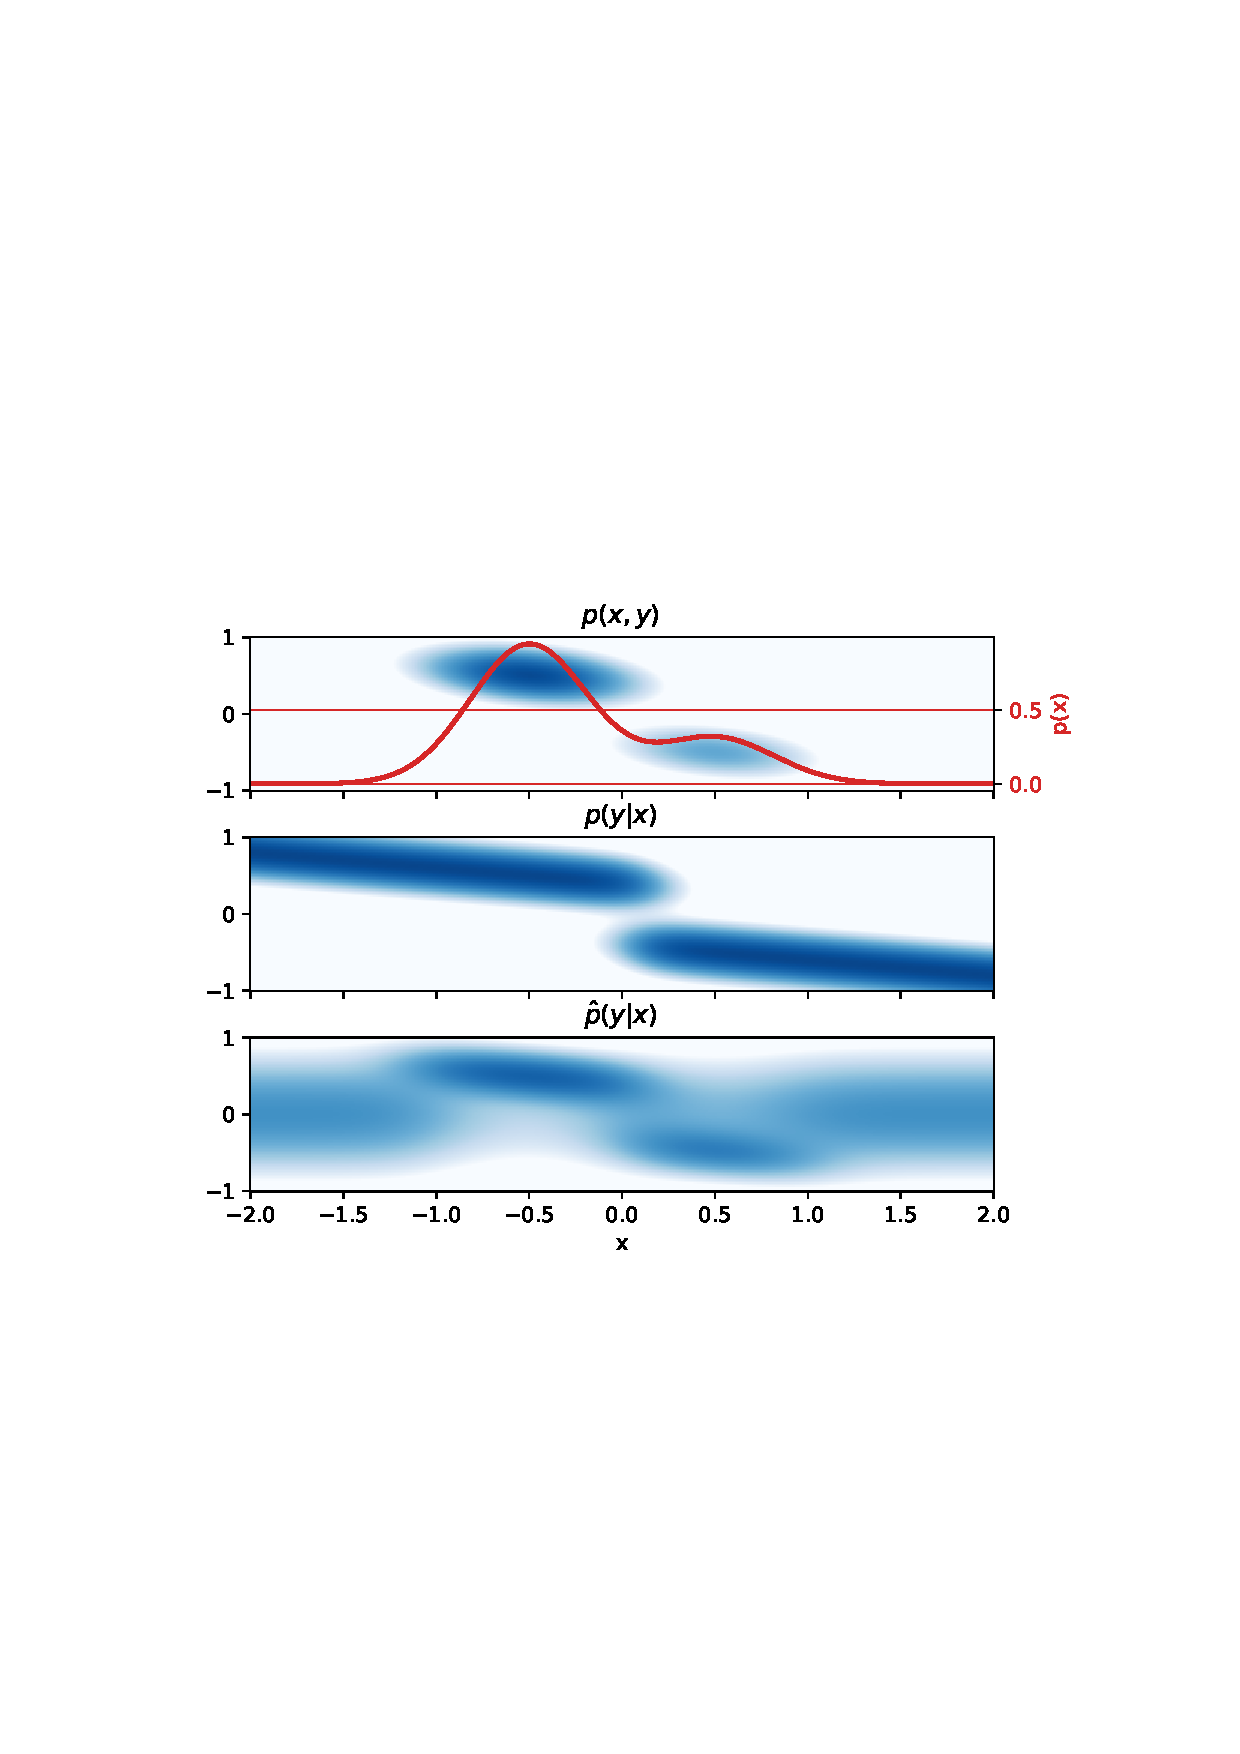
\includegraphics[width=0.45\textwidth]{Pictures/mixture_predictive_bayesian2D.pdf}
    \caption{Left: Illustration of how the preditive distribution is manipulated according
    the the scaling function $S(x) := p(x)\cdot N$. Right: Illustration of why it makes
    sense to manipulate the predictive distribution $p(y|x)$, if there is a small amount of input data
    at a region, then the predictive distribution should collapse into the uncertain prior}
    \label{pred_dist_manipulation}
\end{figure}

\subsubsection{Manipulated predictive mean}
What is the mean prediction of the manipulated predictive distribution?
\begin{align*}
    E_{p_{bayes}(y|x)}[y] &= \int y \cdot \frac{f(n,p(x)) \cdot p(y|x) + \lambda p_{prior}(y)}{Z} dy\\
    &= \left(p(x)\cdot N \cdot E_{p(y|x)}[y] + \lambda \cdot E_{p_{prior}(y)}[y] \right) \frac{1}{Z}\\
    &= \frac{p(x)\cdot N\cdot E_{p(y|x)}[y]}{p(x)\cdot N+\lambda}
\end{align*}

\subsubsection{Manipulated predictive variance}
What is the variance of the manipulated predictive distribution
We first calculate the second moment, 
\begin{align*}
    E_{p_{bayes}(y|x)}[y^2] &= \int y^2 \cdot \frac{p(x)\cdot N \cdot p(y|x) + \lambda p_{prior}(y)}{Z} dy\\
    &= (p(x)\cdot N\cdot E_{p(y|x)}[y^2] + \lambda E_{p_{prior}(y)}[y^2] ) \frac{1}{Z}\\
    &= \frac{p(x)\cdot N \cdot(Var_{p(y|x)}[y]+E_{p(y|x)}[y]^2) + \lambda Var_{p_{prior}(y)}[y]}{p(x)\cdot N+\lambda}
\end{align*}

So the variance is calculated as, 
$$V_{p_{bayes}(y|x)}[y] = E_{p_{bayes}(y|x)}[y^2] - E_{p(x,y)}[y]^2$$

\subsubsection*{implementation}
It is not necessary to calculate the conditional distribution, since, using Bayes rule
$$p(y|x) = \frac{p(x,y)}{p(x)}$$
so gives
$$p_{bayes}(y|x) = \frac{p(x)\cdot N \cdot p(y|x) + \lambda p_{prior}(y)}{Z} = \frac{N \cdot p(x,y) + \lambda p_{prior}(y)}{Z}$$

$$E_{p(x,y)}[y] = \int_y \int_x yp(x,y) dx dy = \int_y y p(y) dy = E_{p(y)}[y]$$

